\section{Coin Flips: Convergence in Probability}
We now have sufficient tools from measure theory to get into the first serious topic of probability - limiting theorems. Given a random sequence $(\xi_1, \xi_2, \dots)$ with $\xi_i$ \textit{independently and identically distributed} (i.i.d.), we would like to study the deviation between the empirical mean (or time average) $S_n/n$ (with $S_n = \xi_1 + \dots + \xi_n$) and the actual mean $\E[\xi_1]$ (space average). In particular, do we know anything when $n \to \infty$?\\

In this chapter, we consider our simplest example of random events: flipping $n$ independent unfair coins.

\subsection{Constructing the sample space}
So how do we represent the flipping of $n$ independent unfair coins in the mathematical framework we have built in the previous sections? Let us consider the case of flipping just one coin. Assume the outcomes are 0 and 1 with probability of getting 1 being $p \in (0,1)$. We hope to express this as a random variable $\xi$ with value in $\set{0,1}$ on suitable probability space $(\Omega, \A, \p)$, such that $\p_\xi(\set{0}) = 1-p$ and $\p_\xi(\set{1}) = p$. A more elaborate way to write the above condition is: 
\begin{equation} \label{eq:Bernoulli_pmf}
    \p_\xi(\set{x}) = p^x (1-p)^{1-x}, \quad x = 0,1
\end{equation}
There are several choices of sample spaces we can choose: \\

\begin{itemize}
    \item The natural choice: 
    $$\Omega = \set{0,1}, \; \A = 2^\Omega, \; \p(\set{\omega}) = p^\omega (1-p)^{1-\omega}, \; \xi(\omega) = \omega$$
    \item A more complicated choice: 
    $$\Omega = [0,1], \; \A = \B([0,1]), \; \p(E) = \Leb(E), \; \xi(\omega) = \chi_{(p,1]}(\omega)$$
    with $\lambda$ being the Lebesgue measure. This represents how a computer simulates a flipping of biased coin: first generate a random number $r \in [0,1]$ from uniform distribution (using e.g. the \verb|numpy.random.rand| function in Python), then return $0$ if $r < 1-p$ and $1$ otherwise. 
\end{itemize}

In both cases we see that $\p_\xi(\set{0}) = 1-p$ and $\p_\xi(\set{1}) = p$. In fact, we have shown from LOTUS (theorem \ref{thm:LOTUS}) that the distribution functions (hence expectation etc.) will not depend on our choice of probability spaces and random variables, as long as $\p_\xi$ satisfies \eqref{eq:Bernoulli_pmf}.\\

How can we extend to the experiment of flipping $n$ coins? The wrong way is to assume that $\xi_1, ..., \xi_n$ are on the same sample space $(\Omega, \A, \p)$ such that $\xi_1= ...= \xi_n$, since these random variables really mean flipping a single coin once and recording the result $n$ times. (In particular the random variables are not independent for sure). In fact, it will be hard to write down a large number of independent random variables defined on any of the sample spaces $(\Omega, \A, \p)$ in the above example. \\

A standard way of describing $n$ independent coin flips (or $n$ independent trials in general) is to assume that the random variables $\xi_1, \xi_2, ..., \xi_n$ in different sample spaces (i.e. $\xi_1$ defines on $(\Omega_1, \A_1, \p_1)$, $\xi_2$ defines on $(\Omega_2, \A_2, \p_2)$ and so on...) However, we need a way to understand any operations involving more than one $\xi_i$'s. The way to mitigate is to consider the product space $(\Omega^{(n)}, \A^{(n)}, \p^{(n)}) = \otimes_{i=1}^n (\Omega_i, \A_n, \p_n)$. As a reminder, the sample space of this new probability space is 
\begin{equation*}
    \Omega^{(n)} = \Omega_1 \times ... \times \Omega_n = \set{\omega = (\omega_1,...,\omega_n) \,:\, \forall i, \; \omega_i \in \Omega_i},
\end{equation*}

the new collection of events are
\begin{equation*}
    \A^{(n)} = \sigma(\set{A_1 \times ... \times A_n \,:\, \forall i, \; A_i \in \A_i}) = 2^{\Omega^{(n)}}
\end{equation*}

and the new probability measures are $\p_n$ satisfying 
\begin{equation*}
    \p^{(n)}(A_1 \times ... \times A_n) = \prod_{i=1}^n \p_i(A_i)
\end{equation*}

Then we can define the family of projection function onto the $i$-th component,  $\proj^{(n)}_i: (\Omega^{(n)},\A^{(n)}) \to (\Omega_i, \A_i)$ such that $\proj^{(n)}_i(\omega_1, ..., \omega_n) = \omega_i$. For convenience, we drop the superscript $(n)$ if there is no ambiguity. Notice that the projection functions are measurable, since the preimage of any sets in $\A_i$ is 
$$\proj_i^{-1}(A_i) = \Omega_1 \times ... \times \Omega_{i-1} \times A_i \times \Omega_{i+1}, ..., \Omega_n \in \A^{(n)}$$

Now we can define new random variables $\tilde{\xi}:(\Omega^{(n)}, \A^{(n)}, \p^{(n)}) \to \set{0,1}$ such that $\tilde{\xi}_i(\omega) = \xi_i(\proj_i(\omega))$. These random variables are an accurate description of flipping $n$ coins since:
\begin{enumerate}
    \item The marginal distribution of $\xi_i$, defined as the measure $A \mapsto \p_{\tilde{\xi}_i}(\Omega_1 \times ... \times A \times ... \times \Omega_n)$ satisfies \eqref{eq:Bernoulli_pmf}.
    \item The family $(\tilde{\xi}_i)$ of random variables are independent.
\end{enumerate}

\begin{exercise}
Verify the above assertions.
\end{exercise}

Finally, we want to extend the above construction to $n \to \infty$, i.e. consider the space $(\Omega, \A) = \otimes_{i=1}^\infty (\Omega_i, \A_i)$ on a suitable probability measure $\p$, so that we can discuss large-sample theorems. We want the probability measure to satisfies:
\begin{equation} \label{eq:consistent_result}
    \p\bracket{A_1 \times ... \times A_n \times \Omega_{n+1} \times ...} = \prod_{i=1}^n \p_i(A_i)
\end{equation}

The good news is, such probability measure exists if we use $\Omega_i \equiv \Omega$ and $\A_i \equiv \A$ in our above examples. If we assume the natural choice, then we can safely set
\begin{equation*}
    \p(\set{(\omega_1,\omega_2,...)}) = \prod_{i=1}^\infty p^{\omega_i} (1-p)^{1-\omega_i} = p^{\sum \omega_i} (1-p)^{\sum (1-\omega_i)}
\end{equation*}
since the probability measure is well-defined for all singletons $\set{(\omega_1,\omega_2,...)}$. If we use the example when $\Omega_i = [0,1]$, we can check that our sequence of measures $(\p^{(n)})$ is consistent (see definition \ref{def:consistent_sequence}) and apply the Kolmogorov Extension Theorem (theorem \ref{thm:kolmogorov_extension}) to define $\p$.\\ 

Note the above construction can be generalised to describe a sequence of independent experiments. The above construction means that we need not worried about specifying a single probability space to describe a sequence of independent experiments. As a summary, \textbf{if we want to describe infinite sequence of experiment with underlying distribution $\p_\xi$, we consider the infinite product space $(\R, \B(\R))^{\otimes \infty}$ equipped with the probability measure $\p$ as determined by the Kolmogorov extension theorem, then the projections onto the $i$-th component $\proj_i$ are random variables with distribution $\p_\xi$.} From now on, we abuse notation by not mentioning the underlying probability space, dropping the tilde sign above $\xi$ and interpreting any operations (especially addition) in the above sense.\\

\subsubsection{Radamecher Functions}
There is a third way to construct a \textbf{fair} coin flip without using the Kolmogorov extension theorem. Consider the probability space $([0,1], \B([0,1]), \p)$ with $\p = \lambda$ being the Lebesgue measure. Consider the binary expansions $\omega = 0.\overline{\omega_1 \omega_2 \dots}_2$ of numbers $\omega \in \Omega$, and define random variables $\xi_1(\omega), \xi_2(\omega),\dots$ by putting $\xi_k(\omega) = \omega_k$. We extend these functions so that for all $k$, $\xi_i(1) = 1$. A neater way to express these random variables is: 
\begin{equation}
\xi_k(\omega) = H(\sin 2^k \pi t)
\end{equation}
where $H(t) = \chi_{[0,\infty)}$ is the heavyside function. Since, for all $n \ge 1$ and all $x_1,\dots, x_n$ taking a value $0$ or $1$, 
\begin{align*}
    \{\omega: \xi_1(\omega) = x_1, \dots, \xi_n(\omega) = x_n \} = \bigg\{ \omega: \frac{x_1}{2} + \frac{x_2}{2^2} + \cdots + \frac{x_n}{2^n} \le \omega < \frac{x_1}{2} + \cdots + \frac{x_n}{2^n} + \frac{1}{2^n} \bigg\},
\end{align*}
the $\p-$measure of this set is $\frac{1}{2^n} = \prod_{i=1}^n \p(\xi_n(\omega) = x_n)$. It follows that $\xi_1, \xi_2, \dots$ is a sequence of independent identically distributed random variables with 
\begin{equation*}
    \p(\xi_1 = 0) = \p(\xi_1 = 1) = \frac12.
\end{equation*}
As we will see in later chapters, such construction give rises to some important number theoretic results regarding binary expansion of numbers in $[0,1]$.


\subsection{Weak Law of Large Numbers}
\subsubsection{A high probability statement for coin flips}
Let $S_n = \xi_1 + \dots \xi_n$. Then 
\begin{equation*}
    \E[S_n] = \sum_{j=1}^n \E[\xi_n] = \sum_{j=1}^n(1 \cdot \p_{\xi_j}(\xi_j = 1) + 0\cdot \p_{\xi_j}(\xi_j = 0)) = np.
\end{equation*}
Thus the mean value of $S_n/n$ is equal to $p$. Our central question is: what does $|\frac{1}{n}S_n(\omega) - p|$ converges to for large $n$? Moreover, in what sense we can consider the convergence? It cannot be that
\begin{equation*}
    \bigg|\frac{S_n(\omega)}{n} - p\bigg| \rightarrow 0
\end{equation*}
uniformly/pointwise in $\omega$, because there is always an $\omega$ such that $\xi_i(\omega) = 1$ for all $i$, so $S_n(\omega)/n \equiv 1 \nrightarrow p$, so we must consider a weaker notion of convergence. Before delving into our discussion, let us recall the following observation

\begin{exercise}
Verify that $S_n \sim \sB(n,p)$. Hence show that $\norm{S_n/n - p}^2_{L^2} = \V[S_n/n] = p(1-p)/n \overset{n \to \infty}{\to} 0$.
\end{exercise}

This shows that, in fact, we have $L^2$ convergence. With more careful analysis we show that we actually have $L^p$ convergence for any $p \in [1,\infty)$. By Chebyshev inequality, we also shows that for all $\epsilon > 0$ (fixed)
\begin{equation} \label{eq:Bernoulli_Chebyshev}
    \p\bracket{\abs{\frac{S_n}{n} - p} > \epsilon} \leq \frac{\V[S_n/n]}{\epsilon^2} = \frac{p(1-p)}{n\epsilon^2}
\end{equation}

So for all $\epsilon > 0$ fixed, we can always make the probability $\p\bracket{\abs{S_n/n - p} > \epsilon}$ arbitrary small by choosing sufficiently large $n$. This is known as \textit{convergence of probability}.\\

\begin{unexaminable}
\begin{remark}
*We can make \eqref{eq:Bernoulli_Chebyshev} sharper by considering Chernoff bound. Indeed, we know that the random variable $S_n$ has moment generating function
\begin{equation}
    M_{S_n}(t) = (1-p+pe^t)^n, \quad \forall t \in \R
\end{equation}

so from Chernoff bound, we know for all $t>0$ we have
\begin{align*}
    \p\bracket{\frac{S_n}{n} - p > \epsilon} &= \p\bracket{\exp(t(S_n - np)) > \exp(tn\epsilon)} \\
    &\leq \frac{\exp(-tnp)\E[\exp(tS_n)]}{\exp(tn\epsilon)} \\
    &= \exp\bracket{n \bracket{\ln(1-p+pe^t) - t(p+\epsilon)}} =: \exp(n(\phi(t)-t\epsilon))
\end{align*}
where $\phi(t):= \ln(1-p+pe^t) - pt$. We claim is that $\phi(t)$ is bounded by a quadratic function. We can prove this by bounding the second derivative of $\phi(t)$. Note that
\begin{gather}
    \phi'(t) = -p + \frac{pe^t}{1-p+pe^t} = 1-p-\frac{1-p}{1-p+pe^t} \\
    \phi''(t) = \frac{(1-p)pe^t}{(1-p+pe^t)^2} = \frac{1-p}{1-p+pe^t}\bracket{1-\frac{1-p}{1-p+pe^t}}
\end{gather}
Let $\displaystyle{u(t) = \frac{1-p}{1-p+pe^t}}$. Then clearly $\forall t, \, 0 < u(t) < 1$. Moreover, we see that $\phi''(t) = u(1-u) = -(u-1/2)^2 + 1/4$. Therefore we know for all $t$, $\phi''(t) \in (0,1/4]$. Hence by Taylor Theorem, there exists a $c$ between $0$ and $t$ such that
\begin{equation}
    \phi(t) = \phi(0) + t\phi'(0) + \frac{t^2}{2}\phi''(c) \leq \frac{t^2}{8} 
\end{equation}
Substitute into our Chernoff bound yields
\begin{equation}
    \p\bracket{\frac{S_n}{n} - p > \epsilon} \leq \exp(n(t^2/8 - \epsilon t)) = \exp(n((t-4\epsilon)^2/8 - 2\epsilon^2))
\end{equation} 
So by choosing $t = 4\epsilon$ (such that the RHS) is minimised we yield a much sharper bound:
\begin{equation}
    \p\bracket{\frac{S_n}{n} - p > \epsilon}  \leq \exp(-2n\epsilon^2)
\end{equation}
By symmetry we also obtain 
\begin{equation} \label{eq:Bernoulli_hoeffding}
    \p\bracket{\abs{\frac{S_n}{n} - p} > \epsilon} \leq 2\exp(-2n\epsilon^2)
\end{equation}
We obtain a much sharper bound than \eqref{eq:Bernoulli_Chebyshev} since we now have exponential decay rather than a quadratic decay. The trick of isolating the term $-nt\epsilon$ and bounding $\phi(t)$ by a quadratic function is common, as this can be generalised with any random variables $S_n \in L^\infty(\Omega)$. Such a bound is called a \textit{Hoeffding bound}.
\end{remark}
\end{unexaminable}

\subsubsection{$L^2$ Weak Law of Large Numbers (WLLN)}
Let us study how the weak law of large numbers can be generalised. We first formally define the definition of convergence in probability. The definition holds for not only real-valued random variables, but also random variables taking values in a Polish space $(X,\B(X))$ (equipped with the Borel $\sigma$-algebra) associated with a metric $d$. Recall that a metric space is Polish if it is complete and separable (see remark \ref{rmk:PolishSpace}). 
\begin{definition}
A sequence $\xi_1, \xi_2, \dots $ of random variables from probability space $(\Omega,\F,\p)$ to Polish space $(X,\B(X))$ with metric $d$ converges \textit{in probability}, or \textit{in measure $\p$}, to the random variable $\xi$ (denoted by $\xi_n \xrightarrow{p} \xi$) if for every $\varepsilon > 0$
\begin{equation*}
    \p(d(\xi_n, \xi) > \varepsilon) \rightarrow 0, \quad n\rightarrow \infty.
\end{equation*}
\end{definition}

\begin{exercise}[Properties of convergence in probability] \label{ex:prop_of_conv_in_prob}
Let $(\xi_i)_{i\geq 1}$, $(\eta_i)_{i \geq 1}$ are sequences of random variables on $(\Omega,\F,\p)$, and also let $\xi$, $\eta$ be random variables on $(\Omega,\F,\p)$
\begin{enumerate}
    \item Check that the limit of convergence in probability is almost surely unique: if $\xi_i$ converges in probability to $\xi$ and $\xi'$ then $\xi = \xi'$ almost surely.
    \item Prove that if $\xi_i \overset{p}{\to} \xi$ and $\eta_i \overset{p}{\to} \eta$ then for all real numbers $a,b$ we have $a\xi_i + b\eta_i \overset{p}{\to} a\xi + b\eta$.
    \item Prove that if $\xi_i \overset{p}{\to} \xi$ and $\eta_i \overset{p}{\to} \eta$ then for all real numbers $a,b$ we have $\xi_i \eta_i \overset{p}{\to} \xi \eta$. Notice this is not necessary true if we have $L^p$ convergence. What's wrong with the argument, and can we refine the statements?
    \item (Slutsky's lemma) Show that if $\xi_i \xrightarrow{p} \xi$ and $\eta_i \xrightarrow{p} \eta$ and if $\varphi(x,y)$ is a continuous function, then 
    \begin{equation*}
        \varphi(\xi_i, \eta_i) \xrightarrow{p} \varphi(\xi, \eta).
    \end{equation*}
\end{enumerate}
\end{exercise}

Note that by Markov inequality that if $\xi_n \to \xi$ in $L^p$ ($p\geq 1$, see definition \ref{def:Lp_convergence}), then we must have $\xi_n \xrightarrow{p} \xi$, because
\begin{equation}
    \p(|\xi_n - \xi| > \varepsilon) \leq \frac{\norm{\xi_n - \xi}_{L^p}^p}{\varepsilon^p} \to 0
\end{equation}

Let $\xi_1, \dots, \xi_n$ be a random variables. Denote
\begin{equation*}
    S_n^{(c)} = \sum_{j=1}^n (\xi_j - \E[\xi_j]).
\end{equation*}
Note $\E[S_n^{(c)}] = 0$. How can we fully use Chebyshev inequality to make the assumptions on $\xi_1,...,\xi_n$ as weak as possible? For simplicity, we first assume $\xi_i \in L^2$ such that $\V[\xi_i] \leq C$ for some constant $C$ independent of $i$. Then, if we assume that $\xi_1,...,\xi_n$ are pairwise uncorrelated (which is a much weaker assumption than independence), then we have 
\begin{equation}
    \V[S_n] = \sum_{i=1}^n \V[\xi_i] \leq Cn
\end{equation}

and hence we have the following 

% \begin{remark}
% \begin{align*}
%     \p \bigg( \bigg|\frac{S_n}{n} - p \bigg| > \epsilon \bigg) &= \sum_{k : |\frac{k}{n} - p|\ge \varepsilon} \p(S_n = k)
% \end{align*}
% concentrated at $k \sim n p!$. 
% \end{remark}

\begin{theorem}[$L^2$ Weak Law of Large Numbers] \label{thm:WLLN2}
Let $\xi_1, \dots, \xi_n$ be uncorrelated $L^2$ random variables such that $\V[\xi_j] \le C$ for some $C > 0$ and all $n \ge 1$. Then $S_n^{(c)}/n \xrightarrow{p} 0$
\end{theorem}
\begin{proof}
By Chebyshev's inequality and since $\xi_j$ are uncorrelated, for all $\epsilon > 0$
\begin{equation}
    \p  \bigg(\bigg|\frac{S_n^{(c)}}{n}\bigg| > \varepsilon\bigg) \leq \frac{\V[S_n^{(c)}/n]}{\varepsilon^2} \leq 
    \frac{C}{n \varepsilon^2} \overset{n \to \infty}{\to} 0
\end{equation}
\end{proof}

Here we list out some applications to the $L^2$ weak law of large numbers.
\begin{example}[Monte Carlo Integration] \label{eg:Monte_Carlo_L2}
Consider $f$ being a measurable function on $[0,1]$ with \\ $C := \int_0^1 |f(x)|^2 < \infty$ (e.g. $f$ being uniformly bounded by some number $M$). We would like to evaluate the integral
\begin{equation*}
    \theta = \int_0^1 f(x) \, dx,
\end{equation*}
which is often intractable. We note that if $U$ is a random variable on some probability space $(\Omega,\F,\p)$ with uniform  distribution $\mathsf{Unif}[0,1]$, then $\theta = \E[f(U)]$. (Note: a candidate of such random variable would be $U: \omega \in ([0,1],\B[0,1],\Leb) \mapsto \omega$). One may therefore hope to estimate $\theta$ using the following "empirical mean": first define random variables $U_1(\omega), U_2(\omega), ... \iid \mathsf{Unif}[0,1]$ using e.g. construction as detailed in section 4.1, then evaluate the following empirical mean
\begin{equation}
\hat{\theta}_n(\omega) := \frac{f(U_1(\omega))+...+f(U_n(\omega))}{n}
\end{equation}
Then it is quite clear that $\E[\hat{\theta}_n] = \theta$. Moreover, since the random variables $f(U_i)$ are independent, identically distributed with finite variance $\V[f(U_i)] = \E[(f(U_i))^2] - \theta^2 = C-\theta^2 < \infty$, so by $L^2$ WLLN we see that $\hat{\theta}_n(\omega) \overset{n\to\infty}\to \theta$ in probability.
\end{example}

The second example concerns about uniform approximation of a continuous function defined on a compact set (in particular $[0,1]$) using polynomials. It turns out the $L^2$ WLLN for the coin-flip scenario provides an elegant proof for the following Weierstrass approximation theorem.

\begin{theorem}[Weierstrass Approximation Theorem]
Let $C_b([0,1])$ be the set of all bounded continuous functions $f:[0,1]\to \R$. If $f(p) \in C_b([0,1])$, then for all $\epsilon > 0$, there is a polynomial $P(p)$ such that
\begin{equation}
    \sup_{p \in [0,1]} |f(p) - P(p)| < \epsilon.
\end{equation}
This means that the set of all polynomials is dense in $C_b([0,1])$.
\end{theorem}

To prove the theorem, it suffices to construct a sequence of polynomial $f_1, f_2, ...$ such that $f_n(p) \overset{n\to\infty}\to f(p)$ uniformly on $[0,1]$. Our sequence will be the following:
\begin{equation}
f_n(p) = \E\sqbracket{f\bracket{\frac{S_n}{n}}} = \sum_{k=0}^n \sqbracket{{n\choose k} (1-p)^{n-k} p^k} f\bracket{\frac{k}{n}},
\end{equation}

where $S_n$ is as defined in the coin-flip setting as in section 4.1. The motivation comes from a corollary of Slutsky's theorem for convergence in distribution (corollary \ref{cor:prob_implies_dist}), which we will discuss further in the next chapter. Make sure to understand the proof below thoroughly, as we will use the trick of splitting sums in a lot of other proofs.

\begin{proof} 
We note that (check!)
\begin{equation} \label{eq:weierstrass_difference}
    |f_n(p) - f(p)| \leq \sum_{k=0}^n \sqbracket{{n\choose k} (1-p)^{n-k} p^k} \abs{f\bracket{\frac{k}{n}} - f(p)}
\end{equation}
So we want to control the difference $\abs{f\bracket{k/n} - f(p)}$. We know that for fixed $\epsilon > 0$, there is a $\delta > 0$ such that $|x-y|<\delta \implies |f(x)-f(y)| < \epsilon$. We know that for each $k$, we have either (1) $|k/n - p| < \delta$ or (2) $|k/n - p| > \delta$. If case (1) holds, then we have $|f(k/n) - f(p)| < \epsilon$, which is nice. By using Chebyshev inequality (see \eqref{eq:Bernoulli_Chebyshev}), we will see that any $k$ that falls into the case (2) won't contribute too much to the sum in the RHS of \eqref{eq:weierstrass_difference}. That motivates us to split this sum into two parts:
\begin{align*} \label{eq:weierstrass_difference}
    |f_n(p) - f(p)| &\leq \textcolor{orange}{\underbrace{\sum_{\set{k\,|\,|k/n-p|<\delta}} \sqbracket{{n\choose k} (1-p)^{n-k} p^k} \abs{f\bracket{\frac{k}{n}} - f(p)}}_{\mathsf{(A)}}} \\
    &\phantom{=} + \textcolor{violet}{\underbrace{\sum_{\set{k\,|\,|k/n-p|\geq \delta}} \sqbracket{{n\choose k} (1-p)^{n-k} p^k} \abs{f\bracket{\frac{k}{n}} - f(p)}}_{\mathsf{(B)}}}.
\end{align*}
We note that (check again!)
\begin{align*}
    \textcolor{orange}{\mathsf{(A)} < \epsilon \sum_{\set{k\,|\,|k/n-p|<\delta}} \sqbracket{{n\choose k} (1-p)^{n-k} p^k} \leq \epsilon};
\end{align*}
and that $M:= \sup_{p\in[0,1]}|f(p)|$ exists, so that
\begin{align*}
    \textcolor{violet}{\mathsf{(B)} \leq 2M\sum_{\set{k\,|\,|k/n-p|\geq\delta}} \sqbracket{{n\choose k} (1-p)^{n-k} p^k} = 2M\p\bracket{|S_n/n - p| \geq \delta}\leq \frac{2Mp(1-p)}{n\delta^2},}
\end{align*}
Since $p(1-p) = 1/4 - (p-1/2)^2 \leq 1/4$, we see that $ \textcolor{violet}{\mathsf{(B)} \leq 2/(n\delta^2)}$, which converges to zero as $n \to \infty$ uniformly for $p \in [0,1]$. This implies that for a sufficiently large $n$ (depending on $\epsilon$), we have $|f_n(p) - f(p)| < 2\epsilon$, completing the proof.
\end{proof}

\begin{exercise}[$L^2$ Weak Law of Large Number for weakly correlated random variables] Let $\xi_1, \xi_2, ...$ be random variables on a common probability space $(\Omega,\F,\p)$ with $\E[\xi_i] = 0$ and $\E[\xi_i \xi_j] = r_{|i-j|}$, where $(r_k)_{k\geq 1}$ is a sequence of real numbers such that $r_k \overset{k\to\infty}\to 0$. Let $S_n = \sum_{i=1}^n \xi_i$. Show that $S_n/n \overset{n\to\infty}\to 0$ in probability. 
\end{exercise}

\begin{hint}
The idea is to expand 
\begin{equation}
\V\sqbracket{\frac{\xi_1 + ... + \xi_n}{n}} = \frac{1}{n^2} \sum_{i,j=1}^n \E[\xi_i \xi_j]
\end{equation}
and to count how many of the terms $\E[\xi_i \xi_j]$ satisfies $|i-j|=k$. 
\end{hint}

If you have done some time series, then you will know from this exercise that any time average of a moving average or autoregressive $\mathsf{AR}(1)$ processes have time averages converging to zero. 

\begin{unexaminable}
\subsubsection{Weak Law of Large Numbers for uniformly integrable random variables}
How far can we generalise the weak law of large numbers? It is unfortunate that the weak law of large numbers does not hold for any sequences of random variables. Here is an example:
\begin{example}
Consider $\xi_1, \xi_2, ...$ being independent and identically distributed, so that they follow a Cauchy distribution with the following density function
\begin{equation}
f(x) = \frac{1}{\pi(1+x^2)}
\end{equation}
The Cauchy distribution is famously know for $\E[|\xi_1|] = \infty$ and that $\E[\xi]$ being undefined. In Chapter 6, we will show that $(\xi_1 + ... + \xi_n)/n$ continues to be a Cauchy distribution as above, hence does not converge to any mean!
\end{example}

However, we may still generalise the weak law of large numbers a little bit further. To explain the loosen condition on the sequence of random variables, let us first define the notion of uniform integrability:
\begin{definition}[Uniform Integrability]
Consider a family (or sequence) of random variables $\set{\xi_\alpha}_{\alpha \in A}$, defined on a common probability space $(\Omega,\F,\p)$ with $A$ being an index set (e.g. $A = \N$ or $\R_{>0}$). We say that the family $\set{\xi_\alpha}_{\alpha \in A}$ is uniformly integrable if 
\begin{equation}
    \lim_{x \to \infty} \bracket{\sup_{\alpha \in A} \E\sqbracket{|\xi_\alpha| \chi_{\set{|\xi_\alpha| > x}}}} = 0
\end{equation}
\end{definition}

\begin{remark}
This is a slightly stronger condition than $\set{\xi_\alpha}_{\alpha \in A}$ being uniformly $L^1$ bounded. To show that any uniformly integrable families $\set{\xi_\alpha}_{\alpha \in A}$ are uniformly $L^1$ bounded, fix an $\epsilon > 0$, then by definition one can choose sufficiently large $x > 0$ such that $\sup_{\alpha \in A} \E\sqbracket{|\xi_\alpha| \chi_{\set{|\xi_\alpha| > x}}} < \epsilon$. Therefore, we have 
\begin{equation*}
\sup_{\alpha \in A} \E\sqbracket{\abs{\xi_\alpha}} \leq \sup_{\alpha \in A} \E\sqbracket{|\xi_\alpha| \chi_{\set{|\xi_\alpha| > x}}} + \sup_{\alpha \in A} \E\sqbracket{|\xi_\alpha| \chi_{\set{|\xi_\alpha| \leq x}}} \leq \epsilon + x < \infty.
\end{equation*}
To show the converse is false, we consider the random variables $\xi_i(\omega) = i \chi_{[0,1/i]}(\omega)$ on the space $([0,1], \B([0,1]), \Leb)$. The sequence of random variables $(\xi_i)_{i\geq 1}$ is clearly uniformly $L^1$ bounded, but it is also clear that $\lim_{x \to \infty} \bracket{\sup_{\alpha \in A} \E\sqbracket{|\xi_\alpha| \chi_{\set{|\xi_\alpha| > x}}}} \geq 1$, which shows that the converse is false.
\end{remark}

\begin{exercise}
Show that in the following cases, the families $\set{\xi_\alpha}_{\alpha \in A}$ are uniformly integrable:
\begin{enumerate}
\item $\set{\xi_{\alpha}}_{\alpha \in A}$ are $L^p$ bounded.
\item $\xi_{\alpha}$ are identically distributed with $\xi_\alpha \in L^1$.
\end{enumerate}
\end{exercise}

\begin{hint}
For (1) use H\"{o}lder inequality. For (2), split $\xi_\alpha = \xi_\alpha \chi_{|\xi_\alpha|>x} + \xi_\alpha \chi_{|\xi_\alpha|\leq x}$ with a carefully chosen $x$.
\end{hint}

We are now ready to state the WLLN for uniformly integrable random variables.
\begin{theorem}[Weak Law of Large Number for uniformly integrable random variables] Let $(\xi_i)_{i\geq 1}$ be an independent, uniformly integrable sequence of random variables. Then 
\begin{equation*}
\frac{S_n^{(c)}}{n} = \frac{1}{n} \sum_{i=1}^n (\xi_i - \E[\xi_i]) \overset{n\to\infty}\to 0 \quad \text{in probability.}
\end{equation*}
\end{theorem}

\begin{hint}
Without loss of generality, we assume that $\E[\xi_i] = 0$, which is fine by the above remark that the means are uniformly bounded. The reason for introducing the notion of uniform integrability is so that we may use the trick of truncation, which goes as follow: given a random variable $\xi_i$, not necessary integrable. We may choose a sufficiently large number $R>0$ and consider the random variables $\tilde{\xi}_{i,R} = \xi_i \chi_{|\xi_i| \leq R}$. The random variables $\tilde{\xi}_{i,R}$ are mutually independent and are in $\mathcal{L}^\infty(\Omega)$, which, in turn, are in $\mathcal{L}^p$ for all $p \geq 1$. We will show that there is an extremely small probability that $\tilde{\xi}_{i,R} \neq \xi_{i}$, so we may pretty much replace $\xi_{i}$ with $\tilde{\xi}_{i,R}$ and utilise the $L^2$ WLLN. We may even prove something stronger, that 
\begin{equation*}
\frac{S_{n,R}^{(c)}}{n} \overset{n\to\infty}\to 0 \; \text{in} \; L^1, \quad S_{n,R}^{(c)} = \sum_{i=1}^n (\xi_{i,R} - \E[\xi_{i,R}])
\end{equation*}
\end{hint}

\begin{proof}
Fix an arbitrary $R>0$. We recall $S_n^{(c)} = \sum_{i=1}^n (\xi_i - \E[\xi_i])$. Then we know that 
\begin{equation*}
\E\abs{S_n^{(c)}/n} \leq \E\abs{S_{n,R}^{(c)}/n} + \E\abs{\bracket{S_n - S_{n,R}}^{(c)}/n}
\end{equation*}
Now note that 
\begin{equation*}
\E\abs{S_{n,R}^{(c)}/n} \overset{\text{(H\"older)}}\leq \sqrt{\E[S_{n,R}^{(c)}]^2}/n \overset{\text{(independence)}}\leq \frac{1}{n} \sqrt{\sum_{i=1}^n \E(\tilde{\xi}_{i,R} - \E[\tilde{\xi_{i,R}}])^2}.  
\end{equation*}
Since $|\xi_{n,R}-\E[\xi_{n,R}]| \leq 2R$, we see that $\E\abs{S_{n,R}^{(c)}/n} \leq 2R/\sqrt{n} \overset{n\to\infty}\to 0$. Finally, 
\begin{align*}
\E\abs{\frac{S_n^{(c)} - S_{n,R}^{(c)}}{n}} &= \frac{1}{n}\E\abs{\sum_{i=1}^n \bracket{\xi_i \chi_{\set{|\xi_i|>R}} - \E\sqbracket{\xi_i \chi_{\set{|\xi_i|>R}}}}} \\
&\leq \frac{2}{n} \sum_{i=1}^n \E|\xi_i \chi_{\set{|\xi_i|>R}}| 
\leq 2 \sup_i \E\sqbracket{|\xi_i| \chi_{\set{|\xi_i|>R}}} \overset{R\to\infty}\to 0
\end{align*}
This shows that $S_n^{(c)}/n \overset{n\to\infty}\to 0$, and hence in probability.
\end{proof}

Therefore, we have the following $L^1$ iid Weak Law of Large Numbers.
\begin{theorem} \label{thm:WLLN1}
Let $\xi_1, \xi_2, ...$ be i.i.d. with $\E|\xi_1|<\infty$. Let $S_n = \sum_{i=1}^n \xi_n$ and $\mu = \E[\xi_1]$. Then $S_n/n - \mu \overset{n\to\infty}\to 0$ in probability.
\end{theorem}

\begin{example}[Monte-Carlo Integration, continued]
Returning to the example \ref{eg:Monte_Carlo_L2}, we see that Monte-Carlo method is still valid for any integrable functions $f \in L^1[0,1]$.
\end{example}

\subsubsection{Triangular Arrays}
We may also look at an array of random variables as arranged below
\begin{equation*}
\begin{array}{ccccc}
    \xi_{1,1} &  &  &  & \\
    \xi_{2,1} & \xi_{2,2} &  &  & \\
    \xi_{3,1} & \xi_{3,2} & \xi_{3,3} &  & \\
    \xi_{4,1} & \xi_{4,2} & \xi_{4,3} &  \xi_{4,4} & \\
    \vdots & \vdots & \vdots & \vdots & \ddots
\end{array}
\end{equation*}
(i.e. $\xi_{n,k}$ with $n$ being row index and $k \in [n] := \set{1,2,...,n}$ being the column index). We would like to know if the sum of rows $S_n = \sum_{k=1}^n \xi_{n,k}$ converges in probability. If the entries in each columns are equal (i.e. $\xi_{m,k} = \xi_{n,k}$ for all $k,m,n$), then we may use WLLN to conclude the convergence. The WLLN can be naturally generalised to the case when the random variables on each row are independent, and we leave the proof as an exercise.
\begin{exercise} \label{ex:L2_WLLN_Array}
Under the above settings, if $\mu_n = \E[S_n], \sigma^2_n = \V[S_n]$ and $\sigma_n^2/b_n^2 \to 0$ then 
\begin{equation*}
\frac{S_n - \mu_n}{b_n} \overset{n\to\infty}\to 0 \quad \text{in} \; L^2 \; \text{and in probability.}
\end{equation*}
\end{exercise}

We may prove the following more general version of the weak law of large numbers for triangular arrays.
\begin{theorem}[Weak Law of Large Number for triangular arrays]
Under the above settings, we let $b_n > 0$ with $b_n \overset{n\to\infty}\to \infty$ and $\tilde{\xi}_{n,k} = \xi_{n,k} \chi_{\set{|\xi_{n,k}| > b_n}}$. Suppose that as $n\to\infty$,
\begin{enumerate}
\item $\sum_{k=1}^n \p(|\xi_{n,k}| > b_n) \overset{n\to\infty}\to 0$, and
\item $\sum_{k=1}^n \E[\tilde{\xi}_{n,k}^2 / b_n^2] \overset{n\to\infty}\to 0$,
\end{enumerate}
then by letting $a_n = \sum_{k=1}^n \E[\tilde{\xi}_{n,k}]$, we have 
\begin{equation*}
\frac{S_n - a_n}{b_n} \overset{n\to\infty}\to 0 \quad \text{in} \; L^2 \; \text{and in probability.}
\end{equation*}
\end{theorem}

\begin{proof}
Let $\tilde{S}_n = \sum_{k=1}^n \tilde{\xi}_{n,k}$. We note that 
\begin{equation*}
\p\bracket{\abs{\frac{S_n - a_n}{b_n}} > \epsilon} \leq \p\bracket{S_n \neq \tilde{S}_n} + \p\bracket{\abs{\frac{\tilde{S}_n - a_n}{b_n}} > \epsilon}
\end{equation*}
The first term of RHS can be bounded by a union bound:
\begin{equation*}
    \p\bracket{S_n \neq \tilde{S}_n} \leq \p\bracket{\bigcup_{k=1}^n \set{\tilde{\xi}_{n,k} \neq \xi_{n,k}}} \leq \sum_{k=1}^n \p(|\xi_{n,k}| > b_n) \overset{n\to\infty}\to 0, 
\end{equation*}
and the second term can be bounded by Chebyshev inequality:
\begin{align*}
\p\bracket{\abs{\frac{\tilde{S}_n - a_n}{b_n}} > \epsilon} \leq \frac{1}{\epsilon^2} \E\abs{\frac{\tilde{S}_n - a_n}{b_n}}^2 \leq \frac{1}{\epsilon^2} \sum_{k=1}^n \frac{\E[\tilde{\xi}_{n,k}^2]}{b_n^2} \overset{n\to\infty}\to 0.
\end{align*}
\end{proof}

As a corollary, we may further weaken the condition of the weak law of large numbers when the random variables $(\xi_i)_{i\geq 1}$ are i.i.d.

\begin{corollary}[Weak Law of Large Numbers for nearly integrable random variables]
Let $\xi_1, \xi_2, ...$ be i.i.d. with $y\p(|\xi|_1 > y) \overset{y\to\infty}\to 0$. Let $S_n = \sum_{i=1}^n \xi_n$ and $\mu_n = \E[\xi_1 \chi_{\set{|\xi_1|\leq n}}]$. Then $S_n/n - \mu_n \overset{n\to\infty}\to 0$ in probability.
\end{corollary}

\begin{proof}
We may apply the WLLN for triangular array with $\xi_{n,k} =: \xi_k$ for all $k \in [n]$ and $b_n = n$. The first condition is satisfied as 
\begin{equation*}
\sum_{k=1}^n \p(|\xi_{n,k}| > n) = n\p(|\xi_1| > n) \overset{n\to\infty}\to 0.
\end{equation*}
To check condition (2), we call the following relationship between moments and tail probability: for all $\xi \in L^2$ we have equation \eqref{eq:exp_p_tail}
\begin{equation}
\E[\xi^2] = \int_0^\infty 2y \p(\xi\geq y) \, dy
\end{equation}
Applying this formula yields:
\begin{equation}
\E[\tilde{\xi}^2_{n,1}/n] = \frac{1}{n}\int_0^\infty 2y\p(|\tilde{\xi}_{n,1}| > y) \, dy = \frac{1}{n}\int_0^n 2y\p(|\tilde{\xi}_1| > y) \, dy
\end{equation}
We finally use dominated (or bounded) convergence theorem to show that this quantity tends to zero as $n\to\infty$. Let $g(y) = 2y \p(|\xi_1| > y)$ for $y\geq 0$. By assumption, we note that $g(y) \overset{n\to\infty} 0$. Since $0 \leq g(y) \leq 2y$ for any $y \geq 0$, we know that $g(y)$ is bounded on any $y \in [0,r]$ for any $r<\infty$, hence on the entire $[0,\infty)$. We also note that
\begin{equation}
    \E[\tilde{\xi}^2_{n,1}/n] = \frac{1}{n} \int_0^n g(y) \, dy = \int_0^1 g(ny) \, dy
\end{equation}
and that $g(ny) \overset{n\to\infty}{\to} 0$ almost surely, so by DCT we have $\E[\tilde{\xi}^2_{n,1}/n] \overset{n\to\infty}\to 0$ as desired.
\end{proof}

\begin{exercise}
Show that the above version of weak law of large numbers implies the $L^1$ WLLN (theorem \ref{thm:WLLN1}).
\end{exercise}

\begin{hint}
Use DCT to check that the required condition is satisfied, and that $\mu_n = \E[\xi_1 \chi_{\set{|\xi_1|>n}}] \overset{n\to\infty}\to \mu$. Then use question 2 in exercise \ref{ex:prop_of_conv_in_prob} to conclude.
\end{hint}
\end{unexaminable}

\subsection{Local and Central Limit Theorem}
We now return to our coin-flipping scenario. Recall we have $S_n = \xi_1 + \xi_2 + \cdots + \xi_n$, where $\xi \iid \mathsf{B}(1,p)$ as constructed in section 4.1. As discussed in previous section, $S_n$ tends to be close to $np$ for large $n$. 
\begin{center}
    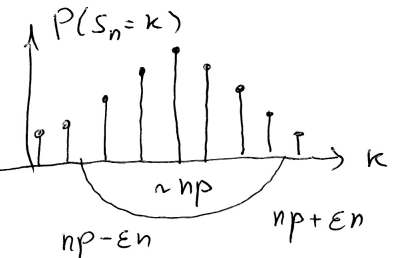
\includegraphics[scale=0.8]{sa.png}
\end{center}

Specifically, let us take some interval $\I_n = (n(p-\varepsilon), n(p+\varepsilon))$. If we pick some sufficiently large $\varepsilon$, say $\varepsilon = n^{\alpha}$ where $\alpha > 1/2$, then by Chebyshev inequality  \eqref{eq:Bernoulli_Chebyshev} (or Hoeffding bound \eqref{eq:Bernoulli_hoeffding}) we know that
\begin{equation} \label{eq:binomial_concentration}
\p(S_n \in \I_n^c) = \p(|S_n/n - p| > n^{\alpha - 1}) \leq \frac{p(1-p)}{n^{1+2\alpha - 2}} = \frac{p(1-p)}{n^{2\alpha - 1}} \overset{n \to \infty}{\to} 0
\end{equation}

and the decaying bounds of $\p(S_n \in \I_n^c)$ no longer exist when $\alpha \leq 1/2$. How much do we know about $\p(S_n \in \I_n^c)$ for this case? Will it tends to some non-trivial constant in $(0,1)$, or will it increase and tend to $1$? We will see that the central limit theorem shows that at the boundary case $\alpha = 1/2$, $\p(S_n \in \I_n^c)$ tends to some non-trivial constant in $(0,1)$ depending on the constant $C$ when defining $\varepsilon = C/n^{1/2}$. This also suggests that the rescaled mean $S_n/n^\alpha$ at the threshold $\alpha = 1/2$ will "converge" in some way to a non-trivial distribution.

\subsubsection{A crash course in asymptotic analysis}
Before we delve into the main discussions, we define two important order notations for sequences $f_n$:

\begin{definition}[Order notations] Consider two sequences $f_n, g_n$. As $n \to \infty$, we say that
\begin{itemize}
    \item (Big $O$) $g_n = O(f_n)$ if $|g_n/f_n|$ is bounded for sufficiently large $n$, i.e. there exists constant $C>0$ and $N$ such that for all $n \geq N$, $|g_n| \leq C|f_n|$
    \item (Small $o$) $g_n = o(f_n)$ if $|g_n/f_n| \to 0$ as $n \to \infty$. In other words, for all constants $\epsilon > 0$, there exists $N := N(\epsilon)$ such that for all $n \geq N$, $|g_n| \leq \epsilon |f_n|$. We also sometimes write $g_n \ll f_n$ or $f_n \gg g_n$.
    \item (Asymptotic equivalence) $g_n \sim f_n$ if $|g_n/f_n| \to 1$ as $n \to \infty$. Equivalently, we have $g_n = (1+o(1)) f_n$.
    \item (Order) $g_n = \Theta(f_n) = \ord(f_n)$ if $g_n = O(f_n)$ but $g_n$ is not $o(f_n)$.
\end{itemize}
\end{definition}

\begin{remark} \phantom{blah} 
\begin{itemize} 
    \item Notice the use of equal sign is an abuse of notation.
    \item The definitions can be extended to any functions $f(x)$ defined on real or complex numbers, in such case we can assume $x$ tends to some points $x_0$ including $\infty$.
    \item We can also consider order notations for sequences of functions. Let $g_n = g_n(\alpha)$, $f_n = f_n(\alpha)$. We say  $g_n(\alpha) = O(|f_n(\alpha)|)$ \textbf{uniformly} if above definition holds with constants $C,N$ independent of $\alpha$. We also have analogous definition for $g_n(\alpha) = o(|f_n(\alpha)|)$.
\end{itemize}
\end{remark}

With this, we can prove one of the most important result in asymptotic analysis
\begin{lemma}[Stirling's Approximation]
As $n \to \infty$, we have
\begin{equation}
    n! = \sqrt{2\pi n} \bracket{\frac{n}{e}}^n \bracket{1 + O(1/n)} 
\end{equation}
\end{lemma}

\begin{unexaminable}
\begin{proof} (Sketch)* There are many ways to prove this famous results, perhaps the quickest way is to notice that $n! = \Gamma(n+1)$, where $\Gamma(z)$ is the Gamma function satisfying
\begin{equation}
    \Gamma(z+1) = \int_0^\infty t^z e^{-t} \, dt = \int_0^\infty \exp(z \ln t - t) \, dt
\end{equation}
Apply a change of variable $s = t/z$, we have
\begin{equation}
    \Gamma(z+1) = \int_0^\infty t^z e^{-t} \, dt = z^{z+1}\int_0^\infty \exp(z(\ln s - s)) \, ds
\end{equation}
Notice the function $\phi(s)$ has the following Taylor series at $s = 1$:
\begin{equation}
    \ln s = \ln (1+(s-1)) = (s - 1) - \frac{(s-1)^2}{2} + O((s-1)^3)
\end{equation}
and therefore
\begin{equation}
    \Gamma(z+1) = z\bracket{\frac{z}{e}}^z \int_0^\infty \exp\bracket{-z \bracket{\frac{(s-1)^2}{2} + O(s-1)^3}} \, dz
\end{equation}
With careful analysis we see that the integral is equivalent to 
\begin{equation}
    \int_{-\infty}^\infty \exp\bracket{-z\frac{(s-1)^2}{2}} \, ds = \sqrt{\frac{2\pi}{z}}
\end{equation}
The main difference is that we now consider range of integration to be $(-\infty, \infty)$ instead of $[0,\infty)$ and ignore the higher order term, in both cases would introduce error which is exponentially small (so can be ignored). Hence we prove that
\begin{equation}
    n! \sim \sqrt{2\pi n} \bracket{\frac{n}{e}}^n
\end{equation}
Refining the analysis to incorporate the $O(1/n)$ correction is hard as it involves more advanced techniques in asymptotic analysis, so will not be included here.
\end{proof}
\end{unexaminable}

With this we can briefly sketch the asymptotic analysis of binomial coefficient. Let's say $n,k,n-k$ all tends to infinity (e.g. $k = np$ for $k \in (0,1)$), then we can use Stirling's formula to obtain
\begin{align*}
    {n\choose k} &= \frac{n!}{k! (n-k)!} \\
    &= \frac{\sqrt{n}}{\sqrt{2\pi k(n-k)}} \frac{(n/e)^n}{(k/e)^k ((n-k)/e)^{n-k}} \textcolor{violet}{\frac{1+O(1/n)}{(1+O(1/n))(1+O(1/n))}}\\
    &= \frac{\sqrt{n}}{\sqrt{2\pi k(n-k)}}  \exp\bracket{n \ln n - k \ln k - (n-k) \ln (n-k)}\textcolor{violet}{\frac{1+O(1/n)}{(1+O(1/n))(1+O(1/n))}}
\end{align*}

We notice that the purple term only gives a correction of $1+O(1/n)$. Instead of going through careful analysis, we can build intuition by treating the $O(1/n)$ correction terms as being exactly equal to $1/n$. Then the denominator satisfies $(1+1/n)^{-2} = 1-2/n+... = 1+O(1/n)$. Then conclude that $(1+1/n)(1-2/n) = 1-1/n+... = 1+O(1/n)$. To sum up, we have
\begin{equation}
    {n\choose k} = \frac{\sqrt{n}}{\sqrt{2\pi k(n-k)}} \exp\bracket{n \ln n - k \ln k - (n-k) \ln (n-k)} \bracket{1+O\bracket{\frac{1}{n}}}
\end{equation}

\subsubsection{Proving the Central Limit Theorem}

We recall the following result regarding the probability mass function of a binomial distribution $\mathsf{B}(n,p)$:
\begin{exercise}[Monotonicity of Binomial probability] \label{ex:mono_of_bin_prob}
Show that $\p(S_n = k)$ is monotone in $k$ below and above its point of maximum.
\end{exercise}

With this we can prove the local limit theorem, which specifies the local asymptotics of probability mass distribution at the point $S_n = k$.

\begin{theorem}[Local Limit Theorem]
For any $0 < p < 1$,
\begin{equation}
    \max_{0 \le k \le n} \bigg|  \p(S_n = k) - \frac{1}{\sqrt{2 \pi p (1-p)} \sqrt{n}} e^{-\frac{x^2}{2p(1-p)}}  \bigg| = o\bigg(\frac{1}{\sqrt{n}}\bigg) \quad n \rightarrow \infty,
\end{equation}
where $\displaystyle{x = x_{k,n} := \frac{k-np}{\sqrt{n}}}$ 
\end{theorem}
\begin{proof}
The main subtlety is that we cannot always apply Stirling's formula. We have to first consider $k$ that are "sufficiently close" to $np$. Specifically, we consider $k$ such that
\begin{equation}
    |x_{k,n}| \leq \frac{A_n}{\sqrt{n}}, \quad A_n = n^\epsilon \; \text{with} \; \epsilon \in (0,1)
\end{equation}
Then we have $k = np+x\sqrt{n}$, $k$
\begin{gather*}
    k = np+x\sqrt{n} = np(1+O(A_n/n))\\
    n-k = n(1-p) - x\sqrt{n} = n(1-p)(1+O(A_n/n))
\end{gather*}
These inequalities ensure that both $k$ and $n-k$ tends to infinity as $n \to \infty$, and we can safely use Stirling's approximation to show that
\begin{align*}
    \p(S_n = k) = \textcolor{orange}{\underbrace{\frac{\sqrt{n}}{\sqrt{2\pi k(n-k)}}}_{\mathsf{(A)}}} \textcolor{violet}{\underbrace{\exp\bracket{n \ln n - k (\ln k - \ln p) - (n-k) (\ln (n-k) - \ln (1-p))}}_{\mathsf{(B)}}} \bracket{1+O\bracket{\frac{1}{n}}}
\end{align*}
We first analyse $\textcolor{orange}{\mathsf{(A)}}$: notice that
\orange{
\begin{align*}
    \mathsf{(A)} &= \frac{\sqrt{n}}{\sqrt{2\pi k(n-k)}} \\
    &= \frac{1}{\sqrt{2\pi np(1-p)(1+O(A_n/n))(1+O(A_n/n))}} \\
    &= \frac{1}{\sqrt{2\pi np(1-p)}} (1+O(A_n/n))
\end{align*}}
The the correction factor can be obtained using similar arguments above. We can then analyse $\textcolor{violet}{\mathsf{(B)}}$ by noticing that 
\textcolor{violet}{
\begin{align*}
    \mathsf{(B)} &= \exp\bracket{n \ln n - k\bracket{\ln n + \ln\bracket{1+\frac{x}{p\sqrt{n}}}} - (n-k)\bracket{\ln n + \ln\bracket{1-\frac{x}{(1-p)\sqrt{n}}}}} \\
    &= \exp\bracket{-\sqbracket{(np+x\sqrt{n}) \ln\bracket{1+\frac{x}{p\sqrt{n}}} + (n(1-p) - x\sqrt{n}) \ln\bracket{1-\frac{x}{(1-p)\sqrt{n}}}}} \\
    &= \exp\bigg( -\bigg[ np\bracket{\frac{x}{p\sqrt{n}} - \frac{x^2}{2p^2 n} + O\bracket{\frac{x^3}{n^{3/2}}} + \frac{x^2}{p} + O\bracket{\frac{x^3}{n^{1/2}}}} \\
    &\phantom{=}+ n(1-p) \bracket{-\frac{x}{(1-p)\sqrt{n}} - \frac{x^2}{2(1-p)^2 n} + O\bracket{\frac{x^3}{n^{3/2}}}} + \frac{x^2}{(1-p)} + O\bracket{\frac{x^3}{n^{1/2}}} \bigg] \bigg) \\
    &= \exp\bracket{-\frac{x^2}{2p(1-p)} + O\bracket{\frac{x^3}{\sqrt{n}}}} \\
    &= \exp\bracket{-\frac{x^2}{2p(1-p)} + O\bracket{\frac{A_n^3}{n^2}}}
    = \exp\bracket{-\frac{x^2}{2p(1-p)}}\bracket{1+O\bracket{\frac{A_n^3}{n^2}}}
\end{align*}
}
Combining, we have
\begin{equation}
    \p(S_n = k) = \frac{1}{\sqrt{2\pi p(1-p)n}} \exp\bracket{-\frac{x^2}{2p(1-p)}} \bracket{1+O\bracket{\frac{A_n}{n}}+O\bracket{\frac{A_n^3}{n^2}}}
\end{equation}
We want to select $\varepsilon < 2/3$ for $A^3_n/n^2 \ll 1$. We select $\varepsilon = 7/12$, then $A_n^3/n^2 = n^{-1/4}$ and $A_n/n = n^{-5/12}$, combining yield
\begin{equation} \label{eq:local_limit_x_closed}
    \max_{|x|\leq A_n/\sqrt{n}} \p(S_n = k) = \frac{1}{\sqrt{2\pi p(1-p)n}} \exp\bracket{-\frac{x^2}{2p(1-p)}} \bracket{1+ \underbrace{O\bracket{\frac{1}{n^{5/12}}}}_{=o(1/\sqrt{n})}}
\end{equation}
We are not done yet, since we still have to consider the case when $x_{n,k}$ satisfies $|x| > \frac{A_n}{\sqrt{n}}$. Fortunately both $\p(S_n = k)$ and the Gaussian tails are very small. Specifically,
\begin{align*}
    &\phantom{=} \max_{|x|>A_n/\sqrt{n}} \abs{\p(S_n = k) - \frac{1}{\sqrt{2\pi p(1-p)n}} \exp\bracket{-\frac{x^2}{2p(1-p)}}} \\ 
    &\leq 
    \max_{|x|>A_n/\sqrt{n}} \abs{\p(S_n = k)} + 
    \max_{|x|>A_n/\sqrt{n}} \abs{\frac{1}{\sqrt{2\pi p(1-p)n}} \exp\bracket{-\frac{x^2}{2p(1-p)}}} \\
    &\leq \max\bracket{\p(S_n = \lfloor np+A_n \rfloor), \, \p(S_n = \lceil np-A_n \rceil)} + \frac{1}{\sqrt{2\pi p(1-p)n}} \exp\bracket{-\frac{A_n^2}{2np(1-p)}}
\end{align*}
The bound of first term is a direct application of exercise \ref{ex:mono_of_bin_prob}. Keeping the choice $A_n = n^{7/12}$, we see immediately that the second term is of $o(1/\sqrt{n})$. Now note that 
\begin{equation}
    n^{1/12} - n^{-1/2} = \frac{np+A_n-np-1}{\sqrt{n}} \leq \frac{\floor{np+A_n}-np}{\sqrt{n}} \leq \frac{np+A_n-np}{\sqrt{n}} = n^{1/12}
\end{equation}
so $x_{\floor{np+A_n},k} \sim n^{1/12}$, and this holds similarly for $x_{\ceil{np+A_n},k}$, so the first term is also $o(1/\sqrt{n})$. Combining these results with \eqref{eq:local_limit_x_closed} completes the proof.
\end{proof}

The local limit theorem really tells us that 
\begin{equation}
    \p\bracket{\frac{S_n - np}{\sqrt{n}} = x} = \frac{1}{\sqrt{n}} \sqbracket{ \frac{1}{\sqrt{2 \pi p (1-p)}} e^{-\frac{x^2}{2p(1-p)}} + o(1)} \quad n \rightarrow \infty
\end{equation}

At first glance you may find this result not useful, as it only tells us that the probability decays to zero at a rate of $O(1/\sqrt{n})$. However, since $\displaystyle{\frac{S_n - np}{np(1-p)}}$ seems to converge to a \textit{continuous} distribution, we really should look at the \textbf{density} by ignoring the $1/\sqrt{n}$. The things inside the square bracket suggests that the density function of $n^{-1/2} (S_n-np)$ "converges" to a normal distribution $\mathbf{N}(0,p(1-p))$, which is equivalent to the distribution of  $\displaystyle{\frac{S_n - np}{np(1-p)}}$ converging to standard normal $\mathbf{N}(0,1)$. The above heuristics can be formalised by adding the local probabilities and consider the cumulative distribution function. We therefore arrive the central limit theorem (CLT).

\begin{theorem}[de Moivre-Laplace CLT] \label{thm:deMoivre_CLT}
For any $0 < p < 1$, $x \in \R$, 
\begin{equation*}
    \lim_{n \rightarrow \infty} \p \bigg(\frac{S_n - np}{\sqrt{np(1-p)}} \le x \bigg) = \Phi (x),
\end{equation*}
where 
\begin{equation*}
    \Phi(x) = \int_{-\infty}^x \frac{1}{\sqrt{2 \pi}} e^{-y^2/2} \d y,
\end{equation*}
is the distribution of $\textbf{N}(0,1)$.
\end{theorem}

\begin{proof}
(Sketch) We note that
\begin{align*}
    \p \bigg(\frac{S_n - np}{\sqrt{np(1-p)}} \le x \bigg) 
    &= \p\bracket{S_n \leq np+x\sqrt{np(1-p)}} \\ 
    &= \sum_{k=0}^{\floor{np-n^{7/12}}-1} \p(S_n = k) + \sum_{k=\floor{np-n^{7/12}}}^{\floor{np+x\sqrt{np(1-p)}}} \p(S_n = k)
\end{align*}
Now note that the first term is a sum of polynomial number of terms in exponentially small order $O(\exp{(-n^{1/2})})$, so will vanish as $n \to \infty$. Notice the second term is a Riemann sum: writing $$T_n = \set{k \,|\, \floor{np-n^{7/12}} \leq k \leq \floor{np+x\sqrt{np(1-p)}}}$$ 
we have 
\begin{align*}
    \sum_{k\in T_n} \p(S_n = k) &= \sum_{k\in T_n} \frac{1}{\sqrt{n}} \frac{1}{\sqrt{2 \pi p (1-p)}} \exp\bracket{-\frac{1}{2} \bracket{\frac{k-np}{\sqrt{np(1-p)}}}^2} \\
    &= \sum_{k\in T_n-np} \frac{1}{\sqrt{n}} \frac{1}{\sqrt{2 \pi p (1-p)}} \exp\bracket{-\frac{1}{2} \bracket{\frac{k/\sqrt{n}}{\sqrt{p(1-p)}}}^2}
\end{align*}
Notice this is almost a Riemann sum on a partition of $(-\infty,x]$ with mesh of partition $1/\sqrt{n}$, missing some boundary terms. One can then show that the boundary terms leads to an $o(1)$ contribution, and conclude that
\begin{equation}
    \lim_{n \rightarrow \infty} \p \bigg(\frac{S_n - np}{\sqrt{np(1-p)}} \le x \bigg) = \int_{-\infty}^x \frac{1}{\sqrt{2 \pi}} e^{-y^2/2} \d y
\end{equation}
We will omit the details here.
\end{proof}

\begin{remark}
It also holds, for all $a < b$, we have
\begin{equation}
    \lim_{n \rightarrow \infty} \p \bigg(a \leq \frac{S_n - np}{\sqrt{np(1-p)}} \leq b \bigg) = \int_a^b \frac{1}{\sqrt{2 \pi}} \exp\bracket{-\frac{y^2}{2}} \, \d y
\end{equation}
With careful analysis, we can let $\displaystyle{a = - \epsilon \sqrt{\frac{n}{p(1-p)}}}$ and $\displaystyle{b = \epsilon \sqrt{\frac{n}{p(1-p)}}}$ to conclude that
\begin{equation}
    0 \leq \p\bracket{\abs{\frac{S_n}{n} - p} > \epsilon} = \bracket{\int_{-\infty}^{- \epsilon \sqrt{\frac{n}{p(1-p)}}} + \int_{\epsilon \sqrt{\frac{n}{p(1-p)}}}^{\infty}} \exp\bracket{-\frac{y^2}{2}} \, \d y + o(1)
\end{equation}
By Mill's ratio inequality \eqref{eq:Mill_Ratio_basic}, we can further control the integral by
\begin{equation}
    \p\bracket{\abs{\frac{S_n}{n} - p} > \epsilon} \leq 2 \sqrt{\frac{p(1-p)}{2\pi n\epsilon^2}} \exp\bracket{-\frac{1}{2} \bracket{\frac{n\epsilon^2}{p(1-p)}}} + o(1)
\end{equation}
So the tail probability tends to zero, leading to the WLLN for coin flipping.
\end{remark}

The de Moivre-Laplace CLT demonstrates that the sequence of random variables $\sqrt{n}((S_n/n) - p)$ converges \textit{in distribution} (converges weakly) to a random variable with normal distribution $\mathsf{N}(0,p(1-p))$. We will formally define the notion of weak convergence in chapter 5-6, and prove a generalised version of central limit theorem.

\subsection{Poisson Convergence}
For completion, let us prove another result concerning convergence in distribution.
\begin{theorem}[Poisson distribution]
Fix $k$ and let $p := p(n) \rightarrow 0$ as $n\rightarrow \infty$ s.t. $p(n) \cdot n \rightarrow \lambda >0$. Then 
\begin{equation}
    \p(S_n =k) = \frac{n(n-1)\cdots(n-k+1)}{k!} \bigg(\frac{\lambda}{n} + o\bigg(\frac{1}{n}\bigg)\bigg)^k \bigg(1 - \frac{\lambda}{n} + o\bigg(\frac{1}{n}\bigg) \bigg)^{n-k} \longrightarrow \frac{1}{k!} \lambda^k e^{-\lambda}.
\end{equation}
\end{theorem}

\subsection{Interlude: An overview to upcoming chapters}
Let us give an overview to the upcoming chapters. In previous sections we have discussed $L^p$ convergence and convergence in probability in detail using the coin flip example. In chapter 5-6 we will discuss weak convergence, and in chapter 7 we will discuss almost sure convergence. The concept of almost sure convergence should have been covered in elementary courses in measure theory. If you have not seen it before, here is the formal definition:

\begin{definition}[Almost sure convergence]
A sequence $(\xi_n)_{n\geq 1}$ of random variables on probability space $(\Omega,\F,\p)$ converges $\p$-almost surely to the random variable $\xi$ (denoted by $\xi_n \overset{a.e.}{\to} \xi$) if 
\begin{equation}
    \p\bracket{\set{\omega\,|\, \xi_n(\omega) \overset{n\to\infty}{\not\to} \xi(\omega)}}
\end{equation}
\end{definition}

Further discussions will follow, but having this definition is probably enough for now. It will be useful to note the following implications of convergence, which is summarised by the following figure. The following figure illustrates the implications.

\begin{figure} [H]
    \centering
    \begin{tikzcd}
    & \overset{L^p}{\to} \arrow[Rightarrow, d]  & \\
    \overset{a.e.}{\to} \arrow[Rightarrow, r] & \overset{p}{\to} \arrow[Rightarrow, r] & \overset{d}{\to}
\end{tikzcd}
\end{figure}

The double arrows refer to implications. This means, in particular, that almost sure convergence and convergence in $L^p$ both imply convergence in probability, and convergence in probability implies convergence in distribution. Notice that all these implications cannot be reversed.\\

One should also note that most of the above notions of convergence are related to some metrics. For instance, it is apparent that $L^p$ convergence involves the metric induced by the $L^p$ norm, and we will see in the next chapter that convergence in distribution involves the so-called Levy-Prokhorov metric. The following exercise shows that convergence in probability induces a metric in the space of all random variables.

\begin{exercise}[Metric for convergence in probability] \label{ex:metric_for_conv_in_prob}
Let $\M$ be the set of the real-valued random variables on the probability space $(\Omega,\F,\p)$. Recall the equivalence relation as defined on \eqref{eq:equiv_relation_Lp}, that $\xi\sim \eta$ iff $\xi=\eta$ $\p$-almost everywhere. Define function $d:\M/\sim \times \M/\sim \to \R$ such that
\begin{equation}
    d([\xi]_\sim, [\eta]_\sim) = \E(|\xi-\eta| \wedge 1)
\end{equation}
\begin{enumerate}
    \item Show that $d$ is a \textit{well-defined} metric on $\M/\sim$.
    \item Let $(\xi_n)_{n\geq 1}$ be a sequence in $\M$ and let $\xi$ be an element of $\M$. Show that $([\xi_n]_\sim)_{n\geq 1}$ converges to $[\xi]_\sim$ with respect to this metric iff $(\xi_n)_{n\geq 1}$ converges to $\xi$ in probability.
\end{enumerate}
Note that the notion of metric can be generalised when $\M$ is the set of random variables taking value on a generic Polish space with metric $d$.
\end{exercise}
\newpage